\documentclass{article}
\usepackage[T1]{fontenc}
\usepackage{amssymb,amsmath}
\usepackage{txfonts}
\usepackage{microtype}
\usepackage{xspace}
\xspaceaddexceptions{\%}

% Lists with less spacing between items
\usepackage{paralist}

% For figures
\usepackage{graphicx}
\usepackage{subfig} 

% For citations
\usepackage{natbib}

% For algorithms
\usepackage{algorithm}
\usepackage{algorithmic}

% the hyperref package is used to produce hyperlinks in the
% resulting PDF.  If this breaks your system, please commend out the
% following usepackage line and replace \usepackage{mlp2017} with
% \usepackage[nohyperref]{mlp2017} below.
\usepackage{hyperref}
\usepackage{url}
\urlstyle{same}

% Packages hyperref and algorithmic misbehave sometimes.  We can fix
% this with the following command.
\newcommand{\theHalgorithm}{\arabic{algorithm}}


% Set up MLP coursework style (based on ICML style)
\usepackage{mlp2018}
\mlptitlerunning{SDP Demo \demoNumber  Group (\groupNumber)}
\bibliographystyle{icml2017}


\DeclareMathOperator{\softmax}{softmax}
\DeclareMathOperator{\sigmoid}{sigmoid}
\DeclareMathOperator{\sgn}{sgn}
\DeclareMathOperator{\relu}{relu}
\DeclareMathOperator{\lrelu}{lrelu}
\DeclareMathOperator{\elu}{elu}
\DeclareMathOperator{\selu}{selu}
\DeclareMathOperator{\maxout}{maxout}







\setGroupNumber{15}
\setGroupName{Group 15}
\setProductName{FoozBot}
\setLogoFileName{figs/FoozBotLogo.png}

\begin{document} 

\makeSDPTitle{Project Plan}

\begin{abstract} 
We aim to create an augmented Foosball table which enables the user to play against a robot. This will include motors to control the footballers, a camera to track the position of the ball, an algorithm for determining how the players will move, and an automatic scorekeeper. We plan to use object detection to track the ball on the field and use the positional information from this to determine how the algorithm for the robot player will behave. Our aim is to have the bulk of work focused on object detection and designing the game playing algorithm as these are the two key aspects which we foresee being most challenging and most integral to the success of the project. This will also be accompanied by smaller amounts of work on peripheral (but nonetheless important) components such as score tracking and the design of a companion web application. Our aim for the design of the mechanical components is to also allow a user to detach and stow the motorized components, thus allowing the table to be used by two human players should the user wish.
\end{abstract} 

\section{Pitch} 
Our desktop Foosball robot consists of three main components: a camera which detects the position of the ball in play, two mechanical controllers which each attach to one of the handles on a given side of the board to control the "players" in the game, and an algorithm which takes the positional data from the camera and moves the mechanical controllers to kick the ball into the opponents goal while playing against another person. In addition, we aim for the mechanical controllers to be detachable and stow-able to allow for 2 humans to play against one another. Lastly, we will add an automatic score tracker, both to set a win-condition for the algorithm and to give the final product functionality even when 2 humans are playing.

Our project hopes to expand the market for Foosball tables, allowing it to become an engaging single-player game when an individual has no one to play with alongside the well-known and fun two-player game when they do. 

\section{The team} 
\subsection{Rose Sarafilovic}
Outside of general programming skills, Rose is good at coming up with designs for relatively complex mechanical components. She will be working on designing and programming the mechanical parts of the system, which may prove difficult if she is doing so alone. Other team members are willing to work with her on this, but they may need some additional help to begin with. 

\subsection{Douglas Torrance}
Douglas has experience in Java and Python programming, however he has no experience at all in robotics or mechanical engineering. He is willing to learn mechanics and embedded systems skills but will require some training first. He'd also prefer for work to be skewed towards the start of the semester. 

\subsection{Tom Lonergan}
Tom has several years of robotics experience from extra-curriculars, and has spent time working with both C++ and Python in various embedded and general purpose computing contexts. He has limited electronics experience, and no mechanical design or manufacture experience at all. He would prefer work to be skewed towards the start of the semester, but understands that that may not be possible.

\subsection{Arnesh Saha}
Arnesh has experience with Java and Python (mostly computer vision), but is relatively new to robotics and willing to learn more about mechanics, provided he has some training first. He would prefer most of the work to be skewed towards the start of the semester.

\subsection{Dorna Hamed Barghi}
Dorna is an intermediate Java and Python programmer. She has no experience in robotics, electronics or mechanical design, however she's willing to develop her knowledge where needed to best aid the group. Dorna also has a lot of experience working in larger teams and is quite comfortable doing project management. One concern is that due to her lack of knowledge on the manufacturing side, it will be difficult to ascertain how long certain tasks will take. A way to mitigate this is to consult with team members continuously as well as our mentor and PhD expert. 

\subsection{Alexander Milchev}
Alexander has experience with a wide variety of programming languages, coupled with brief background knowledge on design, web development and 3D printing. He is otherwise willing to adapt to the team's needs and pick up any part of the project that requires more attention, learning all relevant skills in the process.

\subsection{Yichun Xiao}
Yichun has experience in Java, C and Python programming, and has several experiences working on team projects. She's also completed some 3D modelling before however has little experience in hardware and robotics. She is willing to develop these skills and try working in different areas of the project if needed. She would prefer work to be skewed towards the end of the semester.

\subsection{Nathan Ross}
Nathan is an intermediate Java and Python programmer, with some experience in web development – using tools such as Laravel and Tailwind CSS. He has very limited experience in robotics and hardware, but is keen to learn. He is also looking forward to developing web and mobile applications to work with the hardware, alongside any other tasks needed to complete the project. 

\subsection{Milena Zhang}
Milena has experience with programming languages including Python, Java, and C, along with experience in using CAD software such as Fusion360 and SolidWorks. She also has some knowledge in electronics but has none in mechanical engineering - something she'd like to learn and build on during the development process. She is willing to work on hardware and electronics, alongside any other tasks needed to complete the project. She would prefer the bulk of the work she does to be skewed towards the start of the semester.

\section{Users} 
In order to market FoosBot to a wider target audience, we must consider the range of needs that different users might have.

In 2022, 8.3 million people in the UK, representing 13\% of the population, said they lived alone\cite{census2021}. FoosBot appeals to the growing demographic of single occupants by alleviating boredom and isolation. Moreover, FoosBot can fulfil the social needs of these individuals by connecting them through an interactive and fun game. In further development, two FoosBots can be potentially wireless connected via the internet, allowing users to play FoosBot remotely with their friend or another random FoosBot user living in another region or country.

FoosBot's capacity for one-player fun will be welcomed by introverts seeking solitary enjoyment at home. They will be able to enjoy their favourite pass-time without the need for social interaction, which can sometimes be perceived as exhausting\cite{helgoe2013introvert} and anxiety-inducing. 

The elderly are also potential users of FoosBot. FoosBot is suitable for them as it requires no intensive movement to play, one can stand or sit in the same position throughout, and can be entertaining without the need for an opponent/companion. 

Children aged three and above are another target group for FoosBot. FoosBot benefits children by contributing to cognitive development\cite{dag2021children}, improving hand-eye coordination\cite{health2023Foosball} and fostering competitive skills. Importantly, it frees carers from having to constantly entertain children under their care, enabling them to work on other tasks. 

Besides attracting individual users, FoosBot may also be purchased by companies either to be placed in offices for employees to use during their downtime or for commercial use (for example, being placed in arcades). 
 
For all the potential users, FoosBot will be a great entertainment source, with numerous mental health benefits like relieving stress and alleviating loneliness. However, FoosBot is a mechanical robot that may be noisy at times. This can be disturbing for our users’ neighbours. Hence, we should take care that the noises generated by FoosBot do not exceed 55dB\cite{king2012noise}. 

\subsection{User Stories}

\textbf{Foosball Table Owner}\\
Wants to:  “be able to play Foosball anytime they want” \\
So that: “they can play Foosball anytime they want”

\textbf{Novice Foosball Player}\\
Wants to: “Practice their skills at home against an opponent with adjustable difficulty”\\
So that: “they can improve their skills so they can have fun playing against others“

\textbf{Experienced Foosball Player}\\
Wants to: “play against an opponent skilled enough to be a challenge”\\
So that: “they can have fun playing Foosball”

\textbf{Team Foosball Player}\\
Want to: “play with their friend but as a team, not against them\\
So that: “they can have fun working as part of a team for a common goal”

\textbf{Children}\\
Want to: “play against an opponent they can win against”\\
So that: “they can have a challenging and fun game”

\textbf{Elderly People}\\
Want to: “play a stimulating but non-strenuous game”\\
So that: “they can keep their brains active and do light physical exercise”

\textbf{Potential Conflicts Amongst Users}: Children, elderly individuals and novices are likely to want their opponent to be fairly unskilled, whereas table owners and experienced Foosball players are likely to want the bot to be more challenging, as they're likely to have higher playing skills themselves. This means that one of our later goals, will be to develop adjustable difficulty levels, so that our product is appealing to all potential users. 

\subsection{Stakeholders}
\textbf{Arcades.} Traditional Foosball tables may be left unused if there aren't enough customers to play with. Having an automated player could ensure that customers could always play this game, increasing profitability. Providing an opponent of a consistent difficulty level provides an incentive to improve scores and keep playing\cite{scoring2017game}.

\textbf{Office for Product Safety and Standards (OPSS).} Since children aged three and above are a target group for FoosBot, we must comply with the Toy Safety Directive 2009/48/EC \cite{toys2023regulations}. Our design must not contain sharp edges, toxic components\cite{toy2023safety}, or exposed wires\cite{safetytipsSG}. 

\textbf{The maintenance team.} This stakeholder will want the design to be as simple as possible to allow for easy maintenance. We aim to keep our design simple and document every detail to make it easy to repair and maintain the robot.

\textbf{Other Companies.} Need recreational facilities that can help their employees relax between breaks. Effective breaks lead to productive workers\cite{albulescu2022give}. FoosBot can give employees a fun time during their hour off and make them more willing to work harder when they get back to their desk.

\section{Impact}
Regarding deployment of “FoozBot”, our team plans to have our product released in online stores primarily, targeted for individuals interested in our particular niche in the market, as currently there are no publicly available Foosball tables which allow for playing opposite a robot. Currently it is anticipated that the Foosball table market will rise in the period between 2023 to 2030 \cite{marketInsight} so we believe there is a good chance for wider success of our product as long as we make it a competitive alternative, offering an extra function at a minimal price increase. Ideally we hope the project to be a big enough success to allow us for further deployment beyond online stores, targeting places such as arcades, bars, board game themed cafes or aiming even higher, being sold at supermarkets or franchised sporting goods stores.

We don’t expect the wider social impact to be quite as significant as for example, life saving medicine discoveries, but our aim is to change the way that people perceive games like Foosball. Many of the games with a reputation of being “social games”, that being games that you’d play mostly on outings with friends, have ways to be played alone as well. With the success of our project we hope to inspire other companies to experiment with the idea of automating one side of games like this to provide people interested in them with an extra option for the cases where they might not have anyone to play with. 

In fact the digitisation and automation of games, such as chess, originally a very popular game that required another person to play against, has already happened and proved majorly successful. With a recent resurgence in Chess.com, a widely available website for chess simulation with options to play against Algorithms of varying difficulties, has given rise to a boom in popularity of the game, exposing a much wider audience to it, even breaking into the top most watched games on streaming platforms like Twitch.com for a period of time in 2021 \cite{twitchTracker}. This is due to both the convenience of it being online and the extra convenience of having the ability to play with an artificial player. Providing the convenience of not requiring an extra player for Foosball can give our product and other such products in the industry a similar popularity boom.

\section{Outcomes}
The main aim of our project is to have a working prototype of our idea. This will be a Foosball table with mechanical controllers on one side of the table which will control the footballers and play against a human opponent. These controllers will also be detachable so that two humans can play against each other, this feature is for the users who would have the device in their home for predominantly single-player use, but who occasionally have another person to play against. The ball will be detected by means of video object detection on the play area by a camera suspended above the board by an unobtrusive stand. The ball position will be translated to coordinates which will then be used to control the player positions of the non-human player as it attempts to beat it's human opponent.  

\subsection{Features}
The following details the main features we aim to have in our final prototype, listed from highest to lowest priority, including some quite aspirational features which will only be attempted if the other features are bug-free and reliable. 
\subsubsection{Ball tracking, player control and playing algorithm} Without these three our concept will fail. 
\subsubsection{Detachable controllers} This is a high priority but not strictly necessary for the functionality of the product. It simply helps with marketability. 
\subsubsection{Score tracker} Using a light gate or pressure plate in the goal-well, we will increment a display which tracks the score for each player.
\subsubsection{A web client (and/or mobile app)} This will keep track of players, their scores and games, possibly allowing players to select difficulty if we have time to implement the difficult level feature. In further development, the app would also allow for the online/virtual playing feature which was mentioned in the discussion of users and their potential wants. 
\subsubsection{Difficulty setting} If possible, we would like there to be optional modes of difficulty for the robot opponent, this may not be delivered if making a robotic opponent takes too long. 
\subsubsection{Ball replacement system} A system which automatically places the ball back on the table after a goal is scored. This will only be implemented if we are more than a week or two ahead of schedule.

\subsection{Measuring success}

 In order to measure the success of the player algorithm, we will have to test it against human opponents, yielding a rough estimate of success for the algorithm, and using that determine a difficulty level to assign to the product. Our main initial aim is for the algorithm to be competitive enough that it can provide a challenge for a casual player. 
 
 The success of the detachable controllers is easily measurable - if they can be detached from the play handles and put in a position where they don’t obstruct a person’s hands, then they are successful. 
 
 The score tracker and web client will both be easy to demonstrate as they can be observed on a score display and a screen. The web client may need a short demonstration to show its functionality. 
 
 The difficulty settings will likely be the most difficult to demonstrate as the differences between the modes will only be felt by someone playing against the robot, and only if there is a significant difference in challenge between the modes.

 \subsection{Design}
 While it is difficult to ascertain exactly what our final robot will look like (one reason being that the design is dependent on the foosball table we end up using) we have created mock-up sketches of some of the mechanics, which we're hoping to formalise into CAD diagrams for our first demo. They are included in the final pages of this document.

 \begin{figure*}[!b]
    \centering
    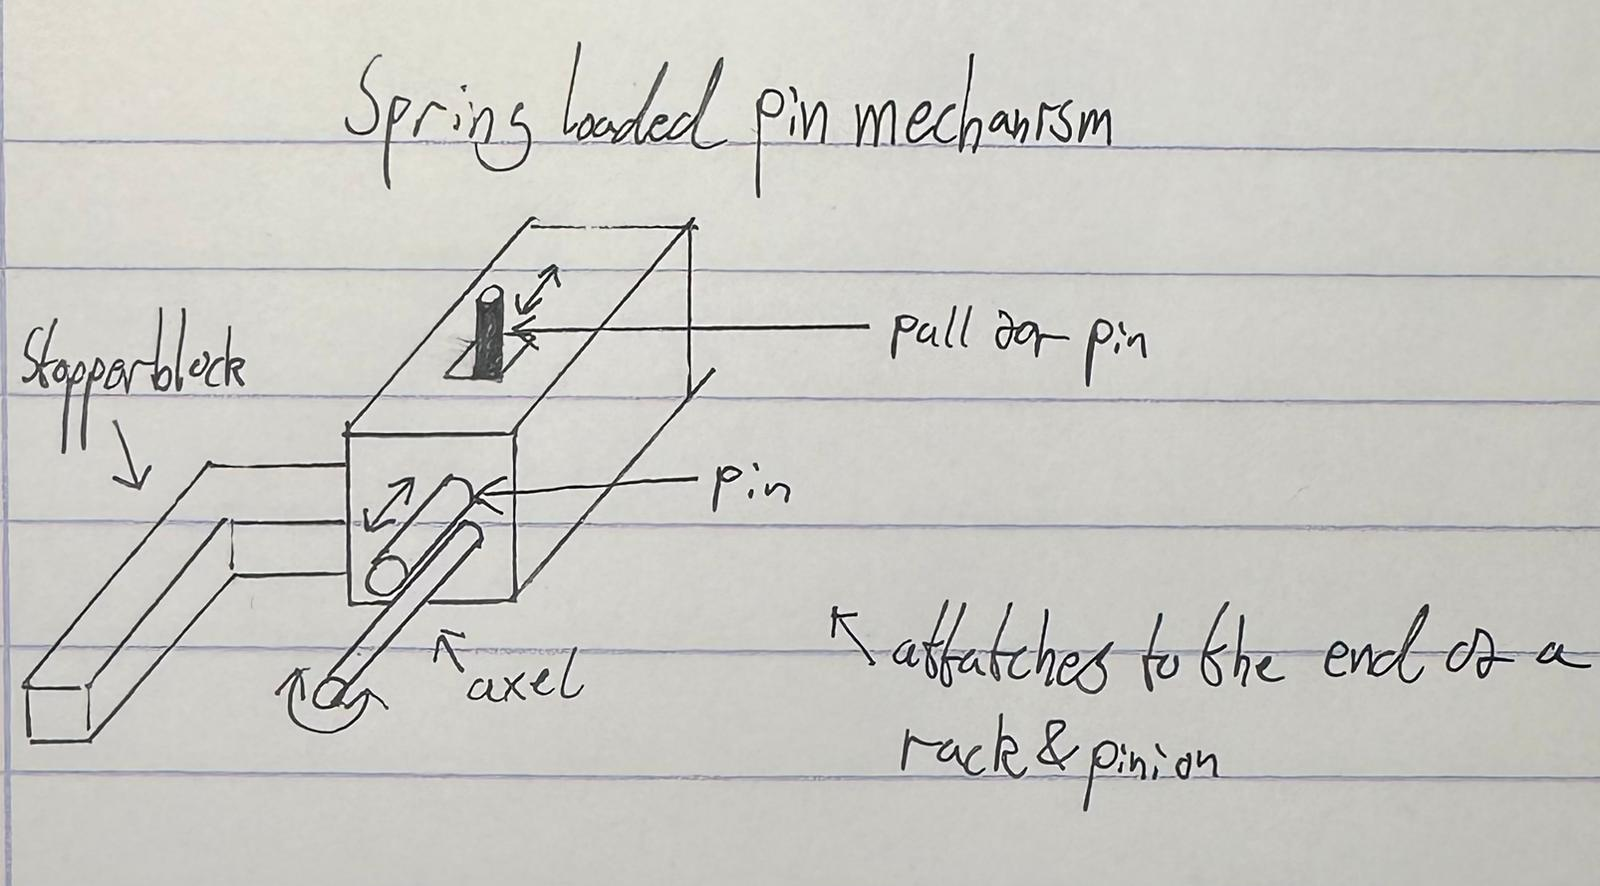
\includegraphics[width=10cm]{figs/design1.jpg}
    \caption{}
    \label{fig:1}
\end{figure*}
 \begin{figure*}[!b]
    \centering
    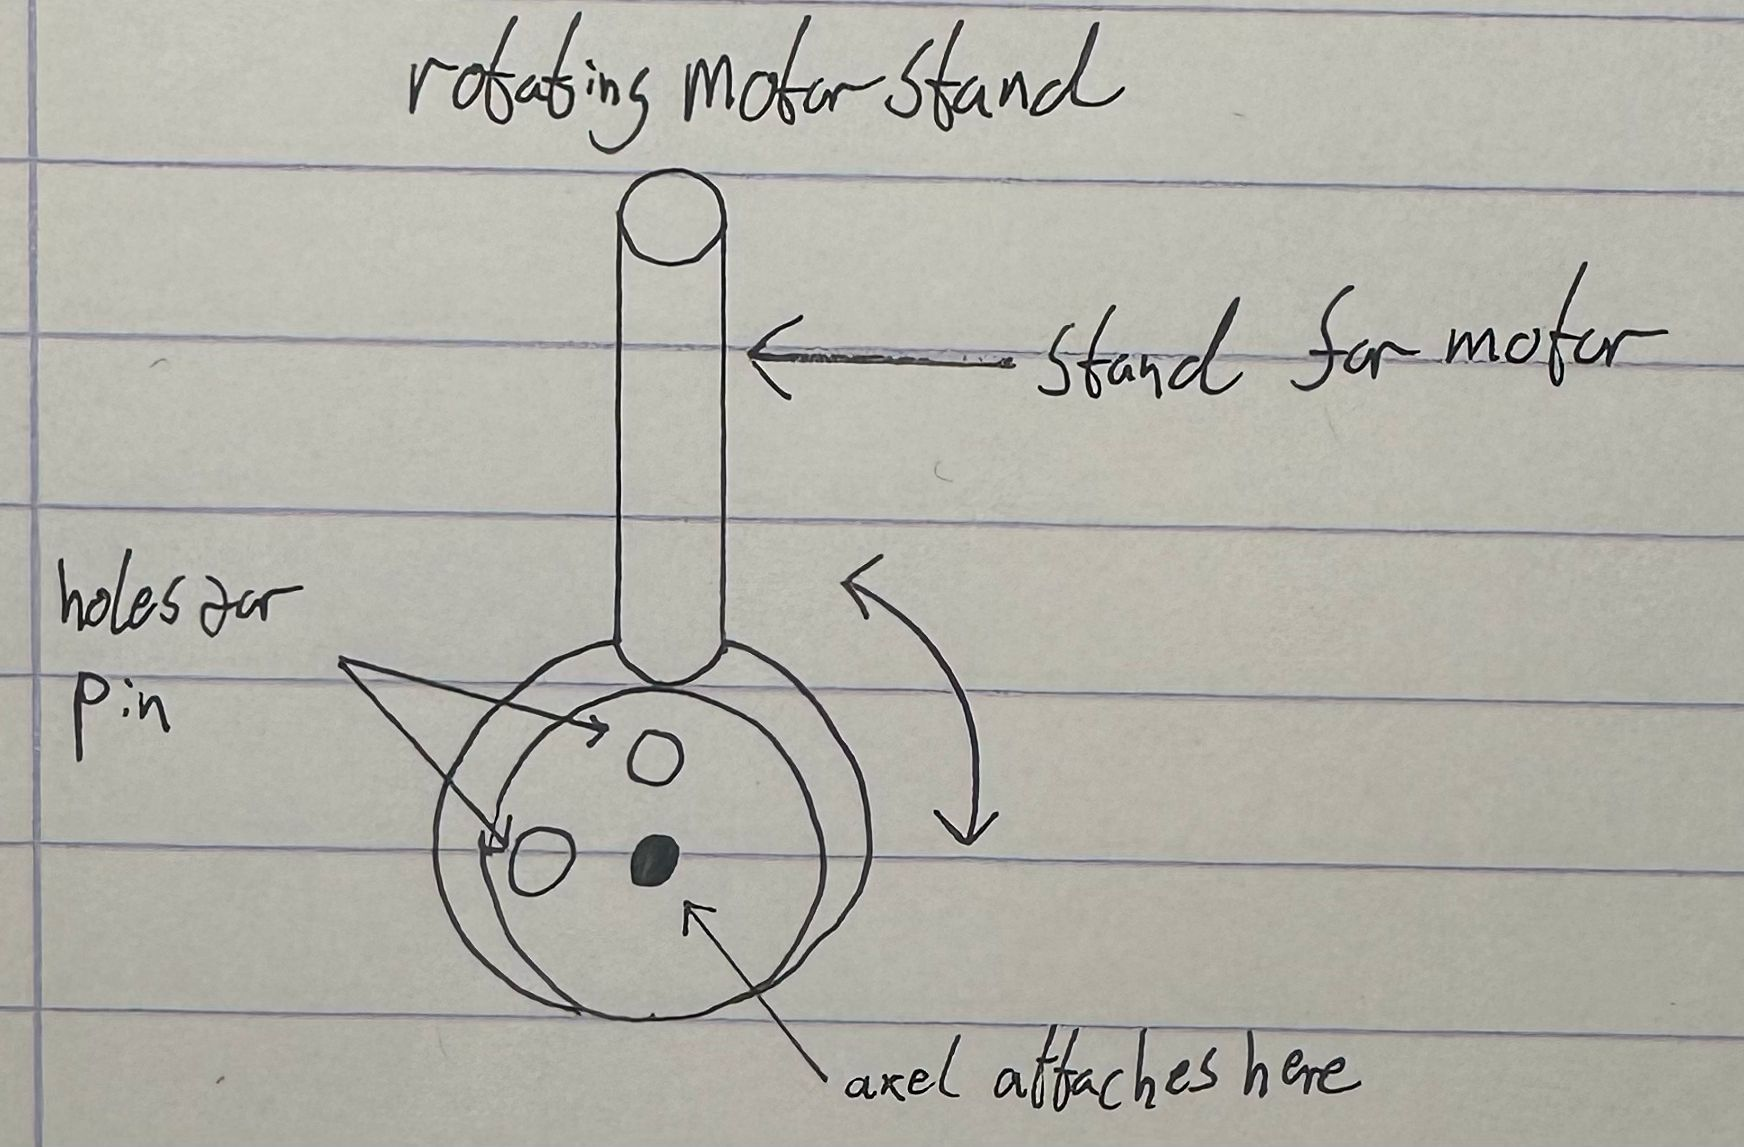
\includegraphics[width=10cm]{figs/design2.jpg}
    \caption{}
    \label{fig:1}
\end{figure*}
 \begin{figure*}[!b]
    \centering
    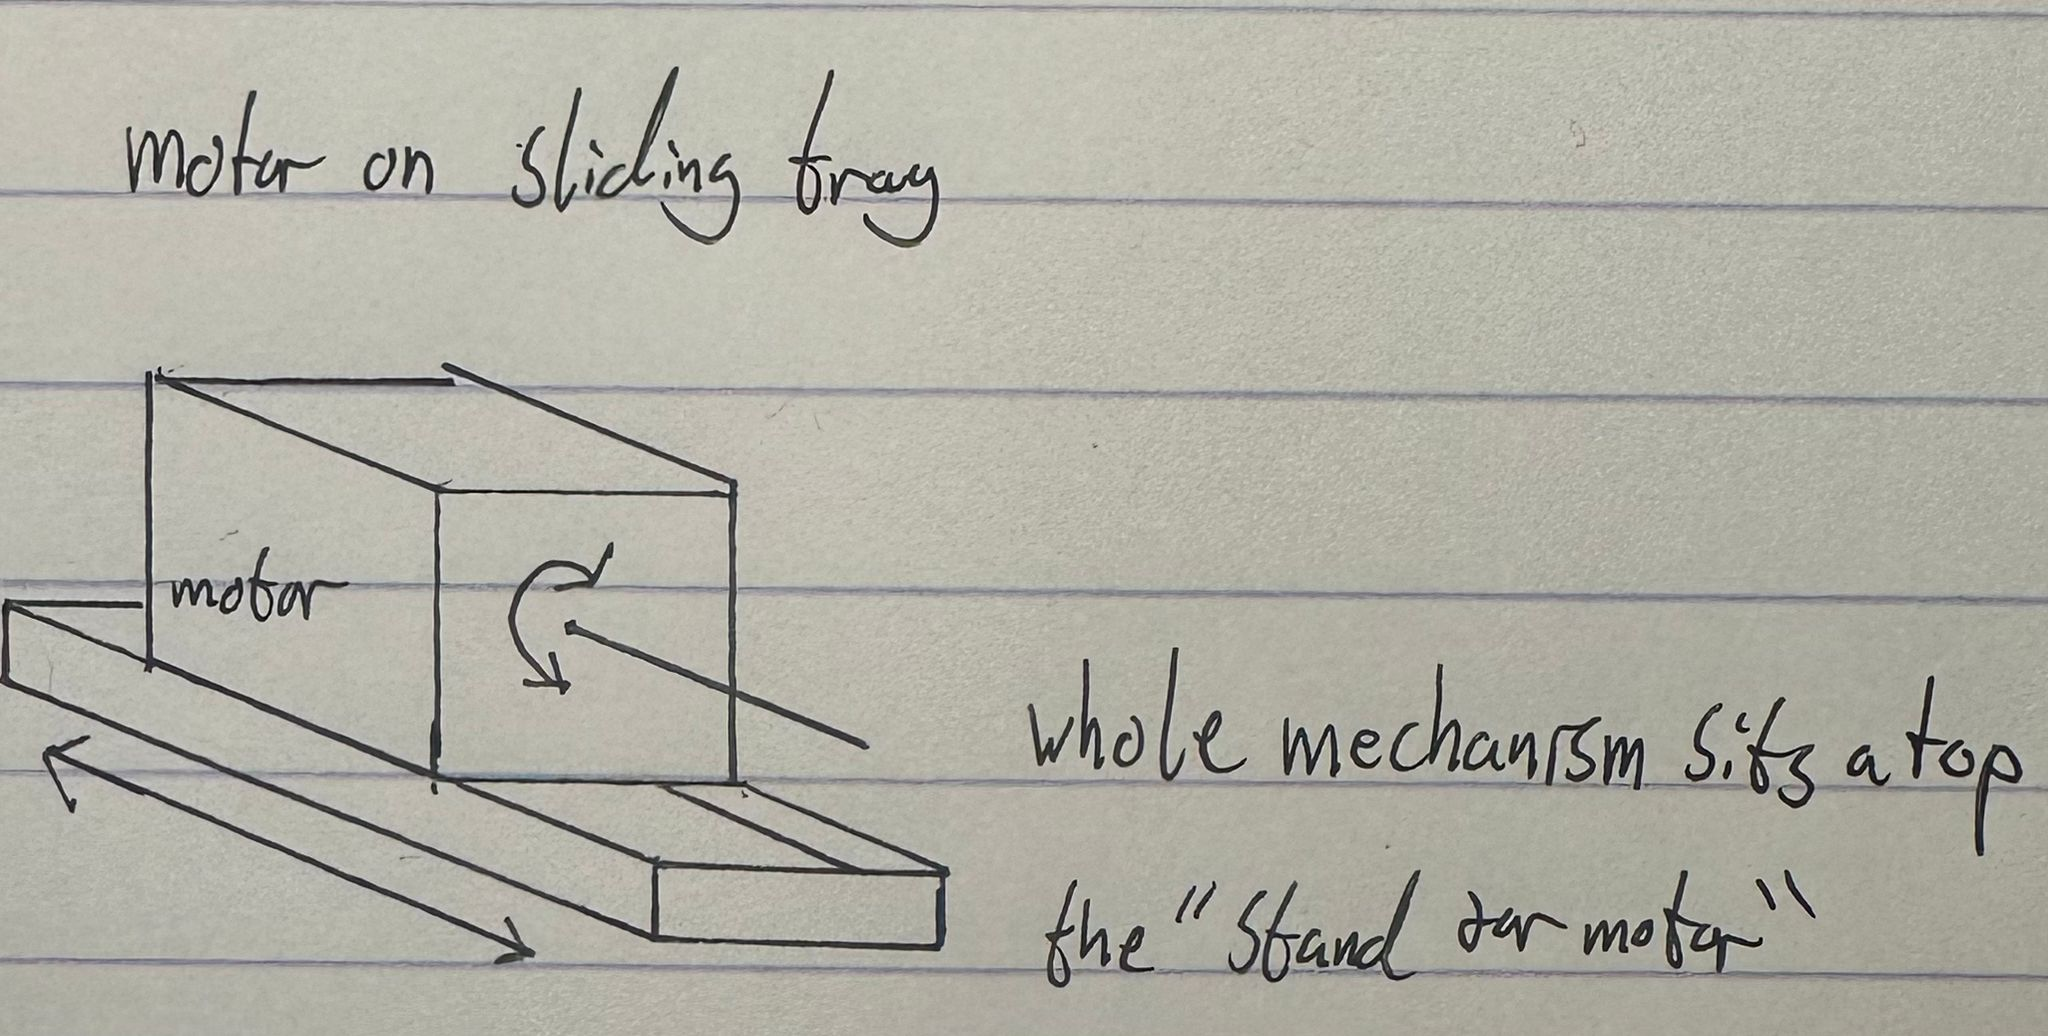
\includegraphics[width=10cm]{figs/design3.jpg}
    \caption{}
    \label{fig:1}
\end{figure*}
 \begin{figure*}[!b]
    \centering
    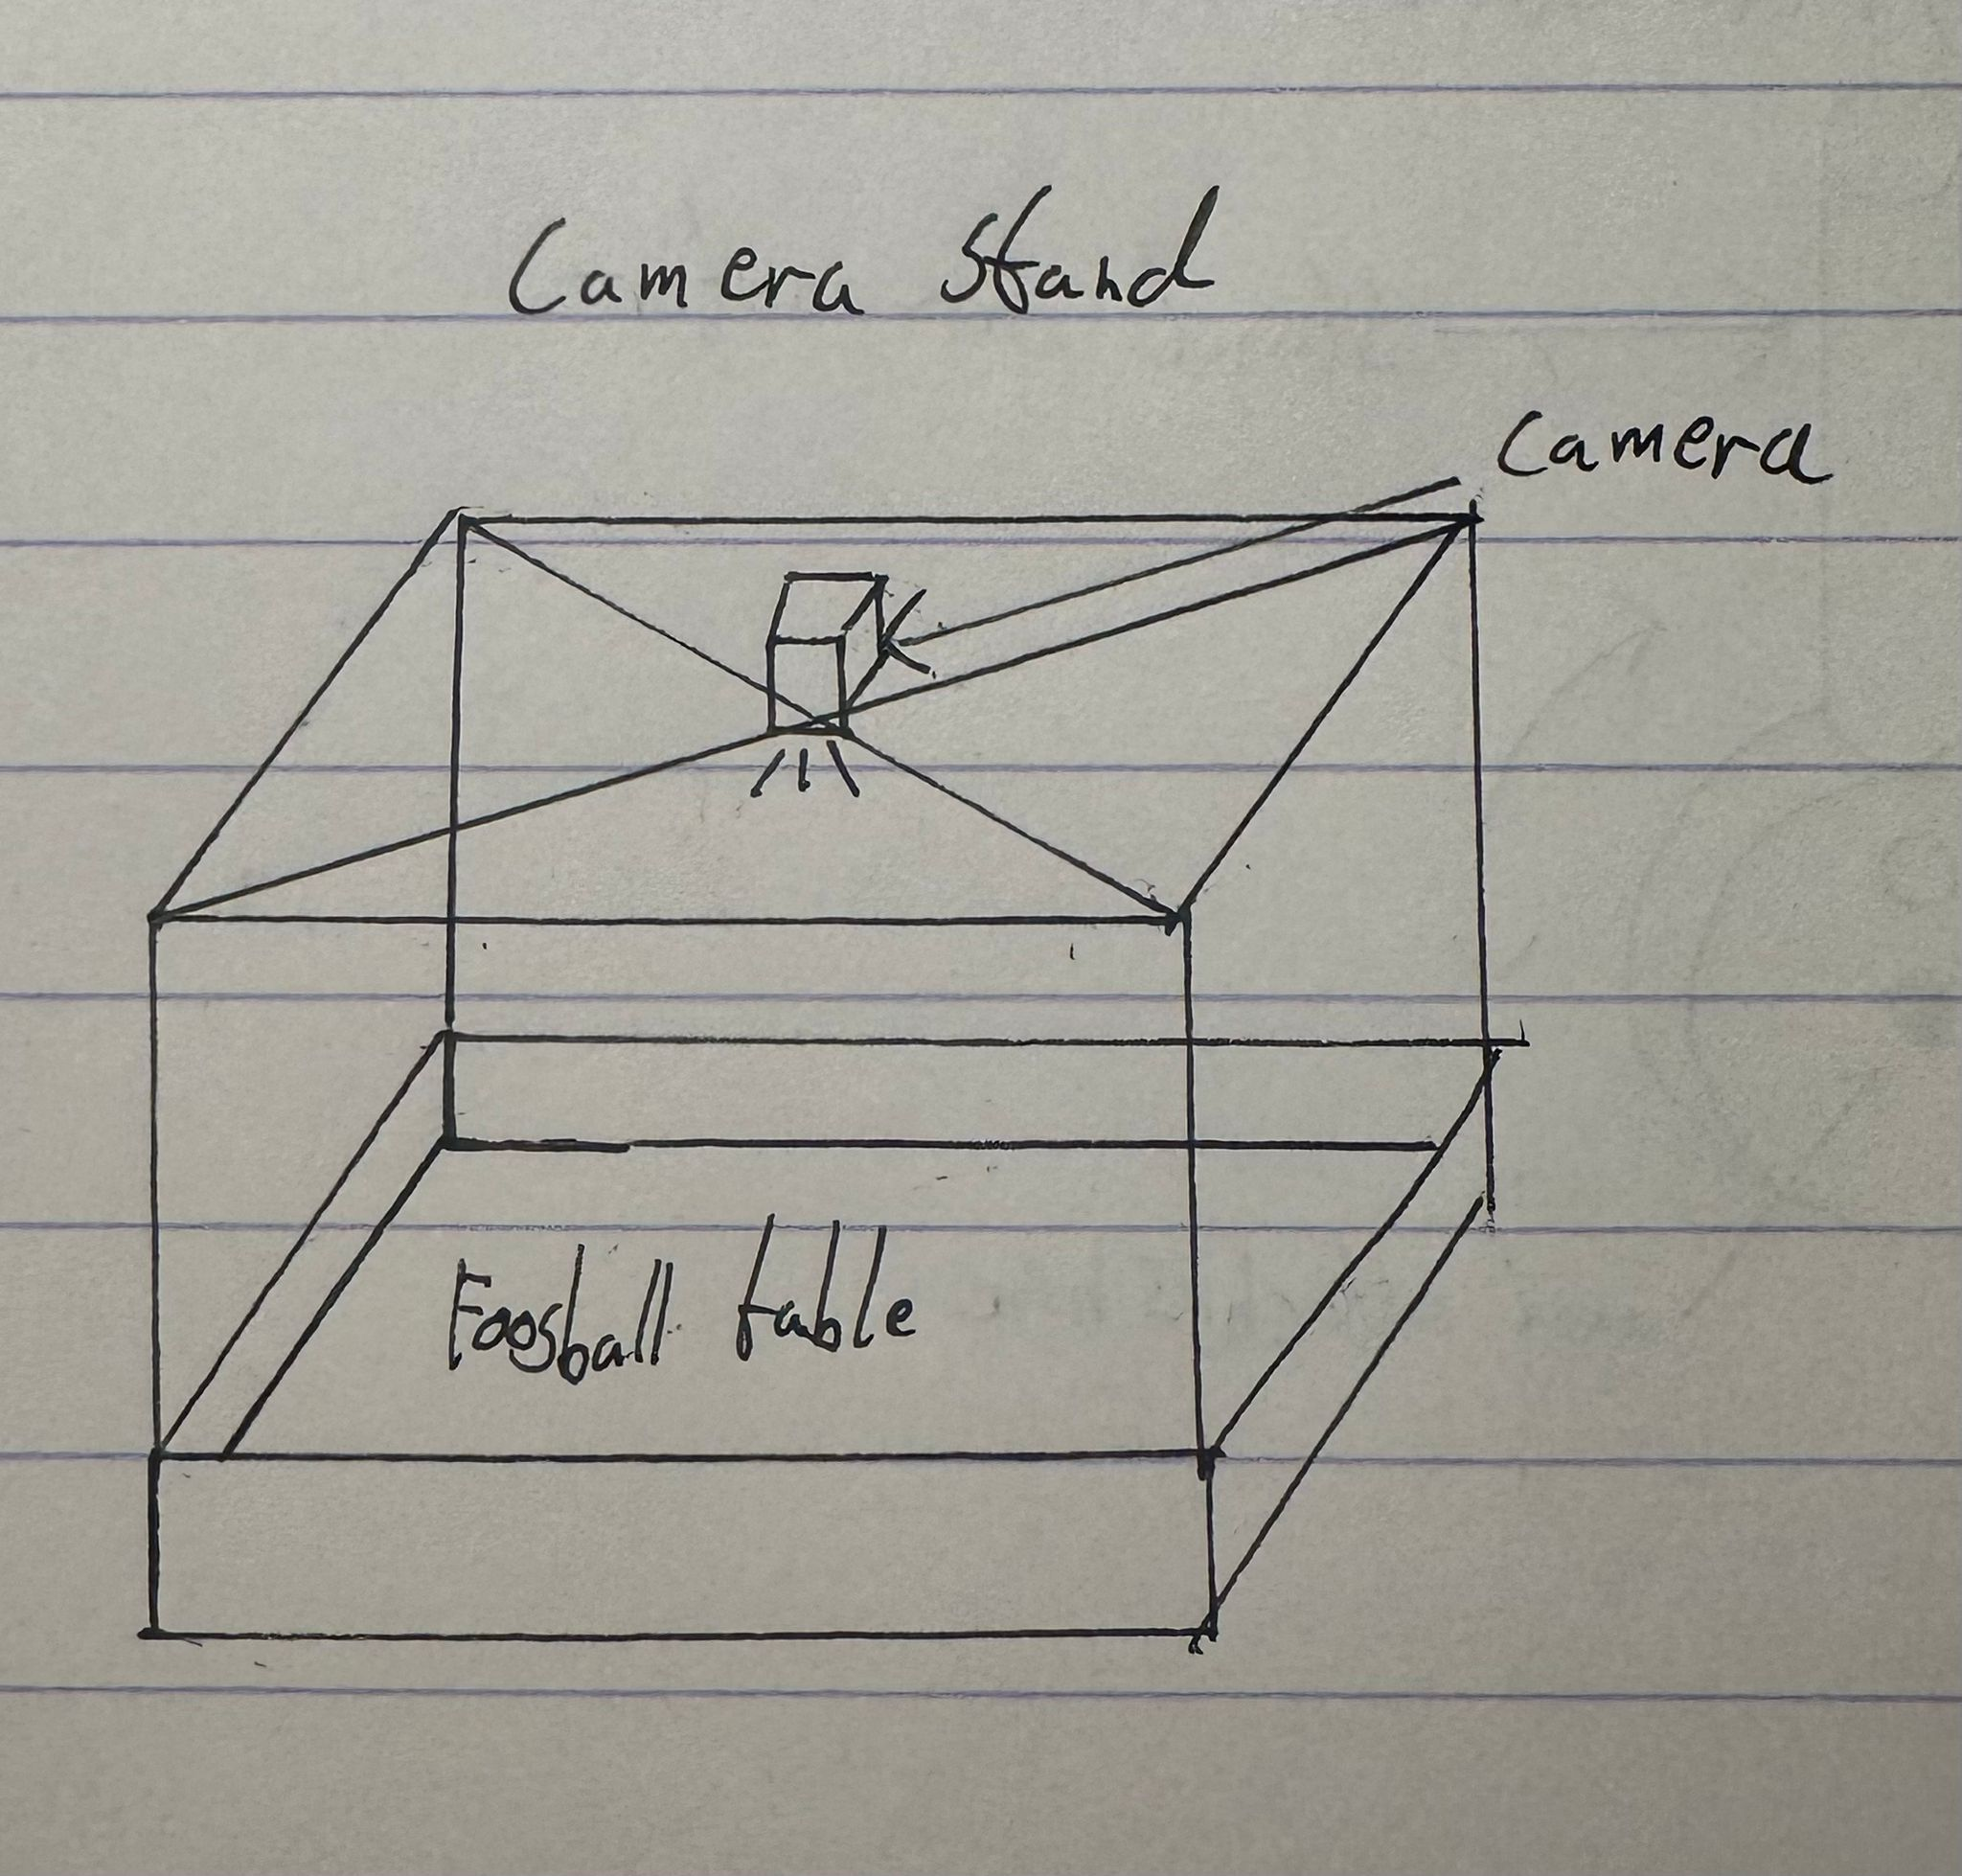
\includegraphics[width=10cm]{figs/design4.jpg}
    \caption{}
    \label{fig:1}
\end{figure*}

\section{Tasks}
\subsection{Subsystems}
Our project can be broken down into the following subsystems.
\subsubsection{Software Development}
\begin{itemize}
    \item Player control algorithm
    \item Ball detection and trajectory prediction
    \item Score tracking
    \item Website/App development
\end{itemize}
\subsubsection{Hardware}
\begin{itemize}
    \item Motor control
    \item Player control
    \item Raspberry Pi set-up
    \item Safety features
\end{itemize}

While a lot of these areas can be completed independently of one another, it is crucial that we begin integrating the system as soon as possible, as this is the area with which we predict we will have the greatest difficulty. 
\subsection{Additional tasks}
In addition to the actual development of the prototype, there are tasks which will require our time. They've been included in the Gantt chart, so that we can ensure we complete them in good time and to a high quality. 
\begin{itemize}
    \item Report write-ups 
    \item Poster/logo design
    \item Market research
\end{itemize}
\subsection{Division of work}
As we've completed our project planning, we've determined that Rose and Milena will focus mainly on the hardware components and that Tom, Yichun and Nathan will be working on the software elements. We've agreed that due to the nature of the project, it will be best for the rest of the members to pick up tasks in whichever areas they're needed, allowing for a more flexible work flow, and better efficiency. All team members will work on aspects of the report and market research, depending on what kind of knowledge/expertise we find is required when these tasks are broken down further. 

\subsection{Time Management}
Our timeline estimation for development of our prototype can be found in the Gantt chart on the final pages of this document. The following provides an explanation of our duration estimates for some of the more significant tasks. 

Ball position detection will likely take around a week, as although there are solutions using libraries like OpenCV \cite{opencv}, it will likely involve some calibration to get it to work with our specific ball and table.

Ball trajectory prediction will similarly take around a week, as we may need to use a Kalman filter or something similar to clean up the camera position data, along with potentially calculating bounces. We will then use another week to verify that our predictions are realistic, and to tune the prediction to be as accurate as possible.

Player control will take around a week, and involves taking the calculated trajectory and determining which football player it comes closest to and how to move that player to the ball. This will again have another week of verification and testing, to ensure that the best possible plays are attempted.

The app/website will take 4-5 weeks, as we will need to implement many components of it, including data collection, hosting, aesthetics, usability, and possible social/competitive features.

Building player control hardware and the structure of the table will take around 2 weeks each, as we will have to wait for the manufacturing of items as well as likely redesigning and manufacturing at least a couple of components.

System integration is the final step, and will take 2-3 weeks so that we can thoroughly identify and resolve any existing defects and refinements required in order to ensure it is as reliable and entertaining as possible in its final state.
\begin{figure*}[!b]
    \centering
    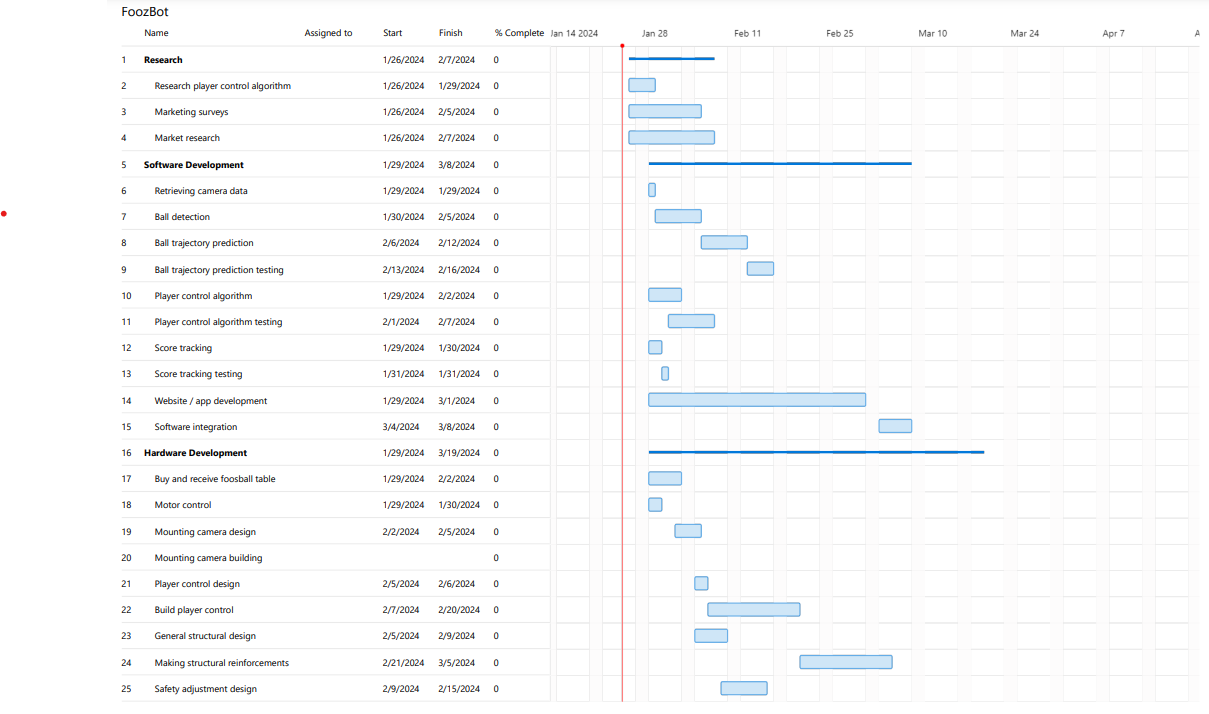
\includegraphics[width=17cm]{figs/project timeline 1.png}
    \caption{Gantt Chart}
    \label{fig:6}
\end{figure*}
\begin{figure*}[!b]
    \centering
    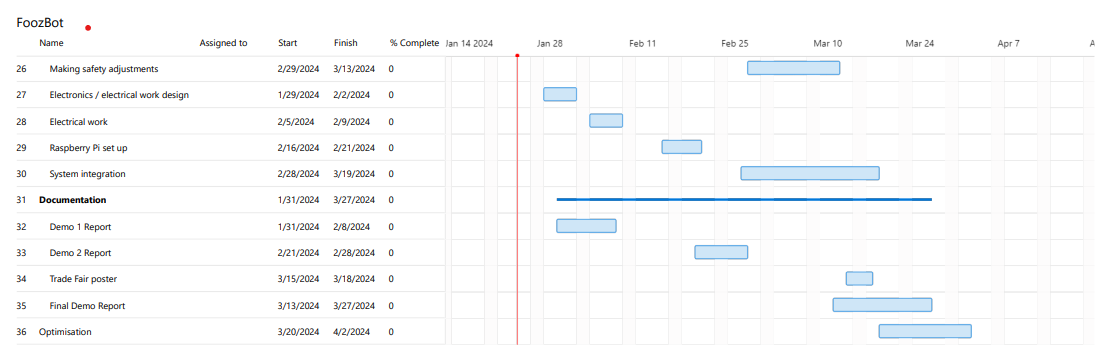
\includegraphics[width=17cm]{figs/project timeline 2.png}
    \caption{Gantt Chart}
    \label{fig:7}
\end{figure*}

\subsection{Demo Goals}
Below we've detailed our goals for our project's progress on each demo day.
\subsubsection{Demo 1}
We have aimed to have market research as well as the majority of research into the player control algorithm to be completed by this time. The code for the motor function will also have been completed. This will include functions for specific commands such as Kick, GoHorizontal, and Stand. These will most likely be demonstrated using a rod attached to the motor player with a plastic rectangular block attached to the rod to imitate the player, and the lateral motion motor will be shown in a similar way, but instead it will simply move a rack and pinion back and forth to specified intervals. On the software side, we aim to have made a detailed design for our web/mobile application, and have completed the ball detection and made a start on the ball trajectory prediction.

\subsubsection{Demo 2}
By the second demo, the fabrication of parts should be completed and thus we can demonstrate the motor functionality on the actual components. This will also likely be linked to the camera and player control algorithm by this point, allowing us to demonstrate how these components will interact. We will have completed the code for the basic functionality of the web/mobile application, and security feature designs will be complete. 

\subsubsection{Peer Demo} At this point we're aiming to have a working prototype with full functionality and thorough testing having been completed on the main features we've set out to implement, including the safety features we've designed. 

\subsubsection{Final Demo} For the final demo, we plan to have integrated the web/mobile application, as well as having completed our integration testing. 

At this point, if we have met all our goals, we will work on optimising our robot as much as possible and working on our more ambitious goals such as enabling difficulty levels.

\subsubsection{Tools}
As is evident through our task breakdown, this project will be very challenging and will require us to be vigilant about our time management, and keep constant track of each subsystems progress. In order to ensure continous communication, we have decided to create a Discord \cite{discord} sever, with separate channels for each subsystem. This means information will be kept relevant and efficient. Additionally, we are making use of Trello \cite{trello} during development to create tickets for tasks, assign them, and keep track of everyone's contributions. 
\section{Risks}
In the development of a competitive Foosball-playing robot, we have identified several key risks. The foremost challenge is the technical complexity and integration of hardware and software components. This encompasses tasks like achieving precise motor control, real-time sensor data processing, and formulating effective AI strategies for various game modes. The failure to seamlessly integrate these aspects could lead to sub-optimal robot performance or complete system failure, undermining the project’s success. To
mitigate this, we plan to conduct rigorous testing of each component before integration, utilize phased integration strategies for optimal compatibility and performance, and implement modular design principles for effective problem isolation and resolution. 

Another significant risk involves hardware failure and safety concerns for developers, owing to the robot's intense physical interaction and proximity to users. Wear and tear of mechanical parts over time, coupled with potential risks from rapid mechanical movements and electrical hazards during development, pose threats to both the product's longevity and developer safety. We intend to counter these challenges by selecting robust, durable materials, establishing regular maintenance schedules, and designing the robot for easy repair and part replacement. Safety measures, such as regulating mechanical speed, ensuring power isolation, and adding protective coverings, will also be crucial to minimize risks.

Finally, the project faces risks related to budget and timespan overruns. The pursuit of high AI accuracy demands precision equipment, which can inflate costs and extend development timelines. Additional features like LED scoreboards and API development further exacerbate this risk. Such overruns could lead to an increased final product price and delayed market entry, potentially impacting customer satisfaction and product competitiveness. Our mitigation strategy here involves prioritizing essential features while scaling back on less critical ones to maintain budget control. In the event of cost overruns, we will focus on revising our marketing strategies to enhance sales and offset the increased expenditure.

Overall, our approach to these risks is dynamic, with continuous monitoring and adaptation being key to our project's success. By proactively managing these challenges, we aim to deliver a robust, entertaining, and safe Foosball-playing robot.

\bibliography{example-refs}

\end{document} 

